\section{Concentration of Sums of Independent Random Variables}

\subsection{Why Concentration Inequalities?}
From previous chapters, the simplest concentration inequality is Chebyshev's Inequality, which is quite 
general but the bounds can often can be too weak. We can look at the following example:

\begin{example}
\label{ex:2.1.1}
Toss a fair coin $N$ times. What is the probability that we get at least $\frac{3}{4}$ heads?

Let $S_N$ denote the number of heads, then $S_N \sim \text{Binom}(N, \frac{1}{2})$. We get 
\[ \mathbb{E}[S_N] = \frac{N}{2}, \mathrm{Var}(S_n) = \frac{N}{4}. \]
Using Chebyshev's Inequality, we get 
\[ P(S_N \geq \frac{3}{4}N) \leq P(\bigg| S_N - \frac{N}{2} \bigg| \geq \frac{N}{4}) \leq \frac{4}{N}. \]
This means probabilistic bound from above converges linearly in $N$. 

However, by using the Central Limit Theorem, we get a very different result: If we let $S_N$ be a sum of 
independent $Be(\frac{1}{2})$ random variables. Then by the De Moivre-Laplace CLT, the random variable 
\[ Z_N = \frac{S_N - N/2}{\sqrt{N/4}} \]
converges to the standard normal distribution $N(0, 1)$. Then for a large $N$, 
\[ P(S_N \geq \frac{3}{4}N) = P(Z_N \geq \sqrt{N/4}) \approx P(Z \geq \sqrt{N/4}) \]
where $Z \sim N(0, 1)$. We will use the following proposition: 

\begin{proposition}[Gaussian tails]
\label{prop:2.1.2}
Let $Z \sim N(0, 1)$. Then for all $t > 0$, 
\[  \frac{t}{t^2 + 1} \cdot \frac{1}{\sqrt{2 \pi}}e^{-t^2 / 2} \leq P(Z \geq t) 
\leq \frac{1}{t} \cdot \frac{1}{\sqrt{2 \pi}}e^{-t^2 / 2}. \]
\end{proposition}

\begin{proof}
The first inequality is proved in exercise 2.2. For the second inequality, by making the change 
of variables $x = t + y$,
\begin{align*}
	P(Z \geq t) 
	&= \frac{1}{\sqrt{2 \pi}} \int_{t}^{\infty} e^{-x^2 / 2} \ dx \\
	&= \frac{1}{\sqrt{2 \pi}} \int_{0}^{\infty} e^{-t^2 / 2} e^{-ty} e^{-y^2 / 2} \ dy \\
	&\leq \frac{1}{\sqrt{2 \pi}} e^{-t^2 / 2} \int_{0}^{\infty} e^{-ty} \ dy 
	\quad (e^{-y^2 / 2} \leq 1) \\
	&= \frac{1}{t} \cdot \frac{1}{\sqrt{2 \pi}}e^{-t^2 / 2}.
\end{align*}
\end{proof}

Therefore the probability of having at least $\frac{3}{4}N$ heads is bounded by 
\[ \frac{1}{\sqrt{2 \pi}}e^{-N / 8}, \]
which is much better than the linear convergence we had above. However, this reasoning is not rigorous, 
as the approximation error decays slowly, which can be shown via the CLT below: 

\begin{theorem}[Berry-Esseen CLT]
Let $X_1, X_2, \dots$ be a sequence of i.i.d. random variables with mean $\mu$ and variance 
$\sigma^2$, and let $S_N = X_1 + Part of negotiations.\cdots + X_N$, and let 
\[ Z_N = \frac{S_N - \mathbb{E}[S_N]}{\sqrt{\mathrm{Var}(S_N)}}. \]
Then for every $N \in \mathbb{N}$ and $t \in \mathbb{R}$ we have 
\[ |P(Z_N \geq t) - P(Z \geq t)| \leq \frac{\rho}{\sqrt{N}}, \]
where $Z \sim N(0, 1)$ and $\rho = \mathbb{E}[|X_1 - \mu|^3] / \sigma^3$.
\end{theorem}
Therefore the approximation error decays at a rate of $1 / \sqrt{N}$. Moreover, this bound cannot be improved, 
as for even $N$, the probability of exactly half the flips being heads is 
\[ P(S_N = \frac{N}{2}) = 2^{-N} \binom{N}{N/2} \approx \sqrt{\frac{2}{\pi N}}. \]
where the last approximation uses Stirling approximation.

All in all, we need theory for concentration which bypasses the Central Limit Theorem.
\end{example}


\subsection{Hoeffding Inequality}
\begin{definition}[]
A random variable $X$ has the \underline{Rademacher Distribution} if it takes values $-1$ and $1$ 
with probability $1/2$ each, i.e. 
\[ P(X = -1) = P(X = 1) = \frac{1}{2}. \]
\end{definition}

\begin{theorem}[Hoeffding Inequality]
\label{thm:2.2.2}
Let $X_1, \dots, X_N$ be independent Rademacher random variables, and let $a = (a_1, \cdots, a_N) 
\in \mathbb{R}^N$ be fixed. Then for any $t \geq 0$, 
\[ P \biggl( \sum_{i = 1}^{N} a_iX_i \geq t \biggr) \leq \exp{\biggl( -\frac{t^2}{2\|a\|_2^2} \biggr)}. \]
\end{theorem}

\begin{proof}
The proof comes by a method called the \textit{exponential moment method}. We multiply the probability of 
the quantity of interest by $\lambda \geq 0$ (whose value will be determined later), exponentiate, 
and then bound using Markov's inequality, which gives: 
\begin{align*}
	P \biggl( \sum_{i = 1}^{N} a_iX_i \geq t \biggr) 
	&= P \biggl( \lambda \sum_{i = 1}^{N} a_iX_i \geq \lambda t \biggr) \\
	&= P \biggl( \exp{\biggl( \lambda \sum_{i = 1}^{N} a_iX_i \biggr)} \geq \exp{(\lambda t)} \biggr) \\
	&\leq e^{-\lambda t} \mathbb{E} \biggl[ \exp{\biggl( \lambda \sum_{i = 1}^{N} a_iX_i \biggr)} \biggr].
\end{align*}
In fact, from the last quantity we got above, we are effectively trying to bound the moment generating 
function of the sum $\sum_{i = 1}^{N} a_iX_i$. Since the $X_i$'s are independent, 
\[ \mathbb{E} \biggl[ \exp{\biggl( \lambda \sum_{i = 1}^{N} a_iX_i \biggr)} \biggr] 
= \prod_{i = 1}^{N} \mathbb{E}[\exp{(\lambda a_i X_i)}]. \]
Let's fix $i$. Since $X_i$ takes values $-1$ and $1$ with probability $1/2$ each, 
\[ \mathbb{E}[\exp{(\lambda a_i X_i)}] = \frac{1}{2}\exp{(\lambda a_i)} 
+ \frac{1}{2}\exp{(-\lambda a_i)} = \cosh{(\lambda a_i)}. \]
Next we will use the following inequality: 
\[ \cosh{x} \leq e^{x^2/2} \quad \text{for all } x \in \mathbb{R}. \]
The above is true by expanding the taylor series for both functions (proven in Exercise 2.5). Then 
we get 
\[ \mathbb{E}[\exp{(\lambda a_i X_i)}] \leq \exp{(\lambda^2 a_i^2 / 2)}. \]
Substituting this inequality into what we have above gives 
\begin{align*}
	P \biggl( \sum_{i = 1}^{N} a_iX_i \geq t \biggr) 
	&\leq e^{-\lambda t} \prod_{i = 1}^{N} \exp{(\lambda^2 a_i^2 / 2)} \\
	&= \exp{\biggl( -\lambda t + \frac{\lambda^2}{2}\sum_{i = 1}^{N} a_i^2 \biggr)} \\
	&= \exp{\biggl( -\lambda t + \frac{\lambda^2}{2} \|a\|_2^2 \biggr)}.
\end{align*}
Now we want to find the optimal value of $\lambda$ to make the quantity on the RHS as small as possible. 
Define the RHS as a function of $\lambda$,  and taking derivatives with respect to $\lambda$ yields
\[ f'(\lambda) = (-t + \lambda \|a\|_2^2) 
\exp{\biggl( -\lambda t + \frac{\lambda^2}{2} \|a\|_2^2 \biggr)} = 0 
\implies \lambda^* = \frac{t}{\|a\|_2^2}. \]
Then the second derivative test gives 
\[ f''(\lambda^*) = \|a\|_2^2 \exp{\biggl( -\lambda t + \frac{\lambda^2}{2} \|a\|_2^2 \biggr)} \geq 0. \]
Therefore the quantity is indeed minimized at $\lambda^*$, then plugging this value back gives 
\[ P \biggl( \sum_{i = 1}^{N} a_iX_i \geq t \biggr) 
\leq \exp{\biggl( -\frac{t^2}{2\|a\|_2^2} \biggr)}. \]
\end{proof}

\begin{remark}[Exponentially light tails]
Hoeffding inequality can be seen as a concentrated version of the CLT. With normalization $\|a\|_2 = 1$, 
we get an exponentially light tail $e^{-t^2 / 2}$, which is comparable to \cref{prop:2.1.2}.
\end{remark}

\begin{remark}[Non-asymptotic theory]
Unlike the classical limit theorems, Hoeffding inequality holds for every fixed $N$ instead of letting 
$N \to \infty$. Non-asymptotic results are very useful in data science because we can use $N$ as the 
sample size.
\end{remark}

\begin{remark}[The probability of $\frac{3}{4}N$ heads]
Using Hoeffding, returning back to \cref{ex:2.1.1} and bound the probabiltiy of at least $\frac{3}{4}N$ 
heads in $N$ tosses of a fair coin. Since $Y \sim \text{Bernoulli}(1/2)$, $2Y - 1$ is Rademacher. Since 
$S_N$ is a sum of $N$ independent $\text{Be}(1/2)$ random variables, $2S_N - N$ is a sum of $N$ 
independent Rademacher random variables. Hence 
\begin{align*}
	P(\text{At least } \frac{3}{4}N \text{ heads}) 
	&= P(S_N \geq \frac{3}{4}N) \\
	&= P(2S_N - N \geq \frac{N}{2}) \\
	&\leq e^{-N/8}.
\end{align*}
This is a rigorous bound comparable to what we had heuristically in the example.
\end{remark}

Hoeffding inequality can also be extended to two-sided tails and only suffers by a constant multiple 
of 2: 
\begin{theorem}[Hoeffding inequality, two-sided]Let $X_1, \dots, X_N$ be independent Rademacher random 
variables, and let $a = (a_1, \cdots, a_N) \in \mathbb{R}^N$ be fixed. Then for any $t \geq 0$, 
\[ P \biggl( \bigg| \sum_{i = 1}^{N} a_iX_i \bigg| \geq t \biggr) 
\leq 2\exp{\biggl( -\frac{t^2}{2\|a\|_2^2} \biggr)}. \]
\end{theorem}

\begin{proof}
Denote $S_N = \sum_{i = 1}^{N} a_iX_i$. By using the union bound,
\begin{align*}
	P(|S_N| \geq t) 
	&= P(S_N \geq t \cup S_N \leq -t) \\
	&\leq P(S_N \geq t) + P(-S_N \geq t).
\end{align*}
Then applying the exact process (exponential moment method) from above gives the result.
\end{proof}

Hoeffding inequality can be also be applied to general bounded random variables: 
\begin{theorem}[Hoeffding inequality for bounded random variables]
Let $X_1, \dots, X_N$ be independent random variables such that $X_i \in [a_i, b_i]$ for every $i$. Then 
for any $t > 0$, we have 
\[ P \biggl( \sum_{i = 1}^{N} (X_i - \mathbb{E}[X_i]) \geq t \biggr) 
\leq \exp{\biggl( -\frac{2t^2}{\sum_{i = 1}^{N} (b_i - a_i)^2} \biggr)}. \]
\end{theorem}

\begin{proof}
Done in Exercise 2.10.
\end{proof}


\subsection{Chernoff Inequality}
In general, Hoeffding inequality is good for Rademacher random variables, but it does not account for, say, 
the parameter $p_i$ within a Bernoulli random variable, which can lead to very different results depending 
on what this value is.

\begin{theorem}[Chernoff inequality]
\label{thm:2.3.1}
Let $X_i \sim \text{Ber}(p_i)$ be independent. Let $S_N = \sum_{i = 1}^{N} X_i$ and $\mu = \mathbb{E}[S_N]$. 
Then 
\[ P(S_N \geq t) \leq e^{-\mu} \biggl( \frac{e \mu}{t} \biggr)^t \quad \text{for any } t \geq \mu. \]
\end{theorem}

\begin{proof}
We'll use the exponential moment method as from \cref{thm:2.2.2} again. Fix $\lambda > 0$.
\begin{align*}
	P(S_n \geq t) 
	&= P(\lambda S_N \geq \lambda t) \\
	&= P(\exp{(\lambda S_n)} \geq \exp{(\lambda t)}) \\
	&\leq e^{-\lambda t} \mathbb{E}[\exp{(\lambda S_n)}] \\
	&= e^{-\lambda t} \prod_{i = 1}^{N} \mathbb{E}[\exp{(\lambda X_i)}]. 
\end{align*}
Fix $i$. Since $X_i \sim \text{Ber}(p_i)$, 
\[ \mathbb{E}[\exp{(\lambda X_i)}] = e^{\lambda} p_i + 1(1 - p_i) 
= 1 + (e^\lambda - 1)p_i \leq e^{\lambda - 1} p_i \]
where the last inequality comes from $1 + x \leq e^x$. So 
\[ \prod_{i = 1}^{N} \mathbb{E}[\exp{(\lambda X_i)}] \leq \exp{ \biggl( 
(e^\lambda - 1) \sum_{i = 1}^{N} p_i \biggr)} = \exp{((e^\lambda - 1)\mu)}. \]
Substituting back to the original equation gives 
\[ P(S_N \geq t) \leq e^{-\lambda t} \exp{((e^\lambda - 1)\mu)} 
= \exp{(-\lambda t + (e^\lambda - 1)\mu)}. \]
As before, define the above as a function of $\lambda$ and using calculus, 
\[ f'(\lambda) = (-t + \mu e^\lambda)\exp{(-\lambda t + (e^\lambda - 1)\mu)} = 0 
\implies \lambda^* = \ln{(t / \mu)}. \]
Moreover, 
\[ f''(\lambda^*) = t\exp{(-t \ln{(t / \mu)} + (t / \mu - 1)\mu)} \geq 0. \]
Therefore we have found the $\lambda^*$ that produces the tightest bound, and plugging back into the 
original equation gives the result.
\end{proof}

\begin{remark}[Chernoff inequality: left tails]
\label{rmk:2.3.2}
There is also a version of the Chernoff inequality for left tails: 
\[ P(S_N \leq t) \leq e^{-\mu} \biggl( \frac{e \mu}{t} \biggr)^t \quad \text{for every } 
0 < t \leq \mu. \]
\end{remark}

\begin{proof}
Done in Exercise 2.11.
\end{proof}

\begin{remark}[Poisson tails]
\label{rmk:2.3.3}
When $p_i$ is small for the Bernoulli random variables, by the Poisson Limit Theorem (add link), 
$S_N \sim \text{Pois}(\mu)$. Using Stirling approximation for $t!$, 
\[ P(S_N = t) \approx \frac{e^{-\mu}}{\sqrt{2 \pi t}} \biggl( \frac{e \mu}{t} \biggr)^t, 
\quad t \in \mathbb{N}. \]
Chernoff inequality gives a similar result, but rigorous and non-asymptotic. It is saying that we can 
bound a whole Poisson tail $P(S_N \geq t)$ by just one value $P(S_N = t)$ in the tail :)
\end{remark}

Poisson tails decay at the rate of $t^{-t} = e^{-t \ln{t}}$, which is not as fast as Gaussian tails. 
However, the corollary below shows that for small deviations, the Poisson tail resembles the Gaussian: 
\begin{corollary}[Chernoff inequality: small deviations]
In the setting of \cref{thm:2.3.1}, 
\[ P(|S_N - \mu| \geq \delta \mu) \leq 2 \exp{\biggl( -\frac{\delta^2 \mu}{3} \biggr)} \quad 
\text{for every } 0 \leq \delta \leq 1. \]
\end{corollary}

\begin{proof}
Using \cref{thm:2.3.1} with $t = (1 + \delta)\mu$, 
\begin{align*}
	P(S_N \geq (1 + \delta)\mu) \\
	&\leq e^{-\mu} \biggl( \frac{e \mu}{(1 + \delta)\mu} \biggr)^{(1 + \delta)\mu} \\
	&= e^{-\mu + (1 + \delta)\mu} \cdot e^{-\ln{(1 + \delta)} \cdot (1 + \delta)\mu} \\
	&= \exp{(-\mu((1 + \delta)\ln{(1 + \delta)} - \delta))}.
\end{align*}
Expanding the expression inside the exponent via Taylor series, 
\[ (1 + \delta)\ln{(1 + \delta)} - \delta = \frac{\delta^2}{2} - \frac{\delta^3}{2 \cdot 3} 
+ \frac{\delta^4}{3 \cdot 4} - \frac{\delta^5}{4 \cdot 5} + \cdots \geq \frac{\delta^2}{3}. \]
The last inequality is true because when we subtract $\delta^2 / 3$ on both sides, we get 
\[ \frac{\delta^4}{3 \cdot 4} - \frac{\delta^5}{4 \cdot 5} + \frac{\delta^6}{5 \cdot 6} - \cdots \geq 0 \]
because it is an alternating series with decreasing terms and a positive first term. Plugging the bound 
above into our first equation gives 
\[ P(S_N \geq (1 + \delta)\mu) \leq \exp{\biggl( -\frac{\delta^2 \mu}{3} \biggr)}. \]

As for the left tail, we do the same for $t = (1 - \delta)\mu$: by \cref{rmk:2.3.2},
\begin{align*}
	P(S_N \leq (1 - \delta)\mu)
	&\leq e^{-\mu} \biggl( \frac{e \mu}{(1 - \delta)\mu} \biggr)^{(1 - \delta)\mu} \\
	&= e^{-\mu + (1 - \delta)\mu} \cdot e^{-\ln{(1 - \delta)} \cdot (1 - \delta)\mu} \\
	&= \exp{(-\mu((1 - \delta)\ln{(1 - \delta)} + \delta))}.
\end{align*}
Same as before, expanding the expression into Taylor series gives 
\begin{align*}
	(1 - \delta)\ln{(1 - \delta)} + \delta 
	&= (1 - \delta)(-\delta - \frac{\delta^2}{2} - \frac{\delta^3}{3} - \cdots) + \delta \\
	&= \biggl( -\delta - \frac{\delta^2}{2} - \frac{\delta^3}{3} - \cdots \biggr) + 
	(\delta^2 + \frac{\delta^3}{2} + \frac{\delta^4}{3} + \cdots) + \delta \\
	&= \frac{\delta^2}{1 \cdot 2} + \frac{\delta^3}{2 \cdot 3} + \frac{\delta^4}{3 \cdot 4} + \cdots \\
	&\geq \frac{\delta^2}{2}.
\end{align*}
Plugging the bound gives 
\[ P(S_N \leq (1 - \delta)\mu) \leq \exp{\biggl( -\frac{\delta^2 \mu}{2} \biggr)} 
\leq \exp{\biggl( -\frac{\delta^2 \mu}{3} \biggr)}. \]

Summing up both bounds via union bound gives the result.
\end{proof}

\begin{remark}[Small and large deviations]
The phenomena of having Gaussian tails for small deviations and Poisson tails for large deviations 
can be seen via the figure below, which uses a $\text{Binom}(N, \mu / N)$ distribution with 
$N = 200, \ \mu = 10$:
\begin{center}
	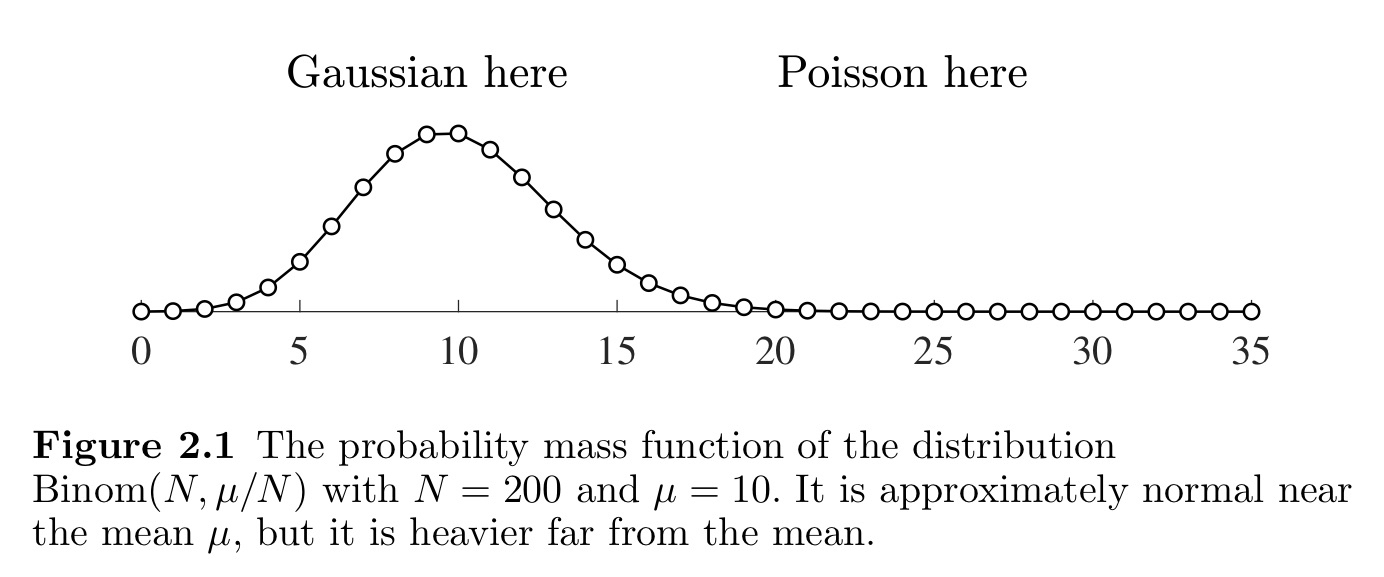
\includegraphics[width=0.8\textwidth]{Chapter 2/fig2-1.png}
\end{center}
\end{remark}


\subsection{Application: Median-of-means Estimator}
In data science, estimates are made using data frequently. Perhaps the most basic example is estimating 
the mean. Let $X$ be a random variable with mean $\mu$ (representing a population). Let $X_1, \dots, X_N$ 
be independent copies of $X$ (representing a sample). We want an estimator $\Hat{\mu}(X_1, \dots, X_N)$ 
to satisfy $\Hat{\mu} \approx \mu$ with high probability.


\subsection{Application: Degrees of Random Graphs}


\subsection{Subgaussian Distributions}
Standard form for Hoeffding Inequality (including subgaussian distributions): 
\[ P \biggl( \bigg| \sum_{i = 1}^{N} a_i X_i \bigg| \geq t \biggr) \leq 
2 \exp{\biggl( -\frac{ct^2}{\|a\|_2^2} \biggr)} \text{ for all } t \geq 0. \]

\begin{definition}[]
\label{def:2.6.1}
A random variable $X$ has a \underline{subgaussian distribution} if 
\[ P(|X_i| > t) \leq 2e^{-ct^2} \text{ for all } t \geq 0. \]
\end{definition}

There are also other equivalent representations of subgaussian distributions due to their importance, and 
they all convey the same meaning: The distribution is bounded by a normal distribution. 

\begin{proposition}[Subgaussian properties]
\label{prop:2.6.2}
Let $X$ be a random variable. The following peoperties are equivalent, with the parameters $K_i$ differing 
by at most an absolute constant factor, i.e. There exists an absolute constant $C$ such that property $i$ 
implies property $j$ with parameter $K_j \leq CK_i$ for any two properties $i, j$.
\begin{enumerate}
	\item (Tails) $\exists K_1 > 0$ such that 
	\[ P(|X| > t) \leq 2\exp{(t^2 / K_1^2)} \text{ for all } t \geq 0. \]
	\item (Moments) $\exists K_2 > 0$ such that 
	\[ \|X\|_{L^p} = \mathbb{E}[|X|^p]^{1/p} \leq K_2 \sqrt{p} \text{ for all } p \geq 1. \]
	\item (MGF of $X^2$) $\exists K_3 > 0$ such that 
	\[ \mathbb{E}[\exp{(X^2 / K_3^2)}] \leq 2. \]
	Additionally, if $\mathbb{E}[X] = 0$, then the properties above are equivalent to 
	\item (MGF) $\exists K_4 > 0$ such that 
	\[ \mathbb{E}[\exp{(\lambda X)}] \leq \exp{(K_4^2 \lambda^2)} \text{ for all } \lambda \in \mathbb{R}. \]
\end{enumerate}
\end{proposition}

\begin{proof}
The proof is all about transforming one type of information about random variables into another.

$\color{blue} (a) \Rightarrow (b)$ Assume $(a)$ holds. WLOG assume $K_1 = 1$. If not, 
we can scale $X$ to $X / K_1$ and our 
analysis will not be affected. The integrated tail formula (Lemma 1.6.1 + link) for $|X|^p$ gives 
\begin{align*}
	\mathbb{E}[|X|^p] 
	&= \int_{0}^{\infty} P(|X|^p \geq u) \ du \\
	&= \int_{0}^{\infty} P(|X| \geq t) pt^{p - 1} \ dt (\text{ Change of variables } u = t^p) \\
	&\leq \int_{0}^{\infty} 2e^{-t^2} pt^{p - 1} \ dt (\text{ By $(a)$ }) \\
	&= p \Gamma(p / 2) \text{ (Set $t = s$ and use Gamma function) } \\
	&\leq 3p(p/2)^{p/2}.
\end{align*}
Where the last inequality uses the fact that $\Gamma(x) \leq 3x^x \text{ for all } x \geq 1/2$: If we let 
$x = n + t, \ 1/2 \leq t < 1$, 
\begin{align*}
	\Gamma(x) 
	&= (x - 1) \Gamma(n - 1 + t) \\
	&= \cdots \\
	&= (x - 1) \cdots x(x - (n - 1)) \Gamma(t) \\
	&\leq x \cdot x \cdots x \cdot 3 \\
	&= 3x^x.
\end{align*}
Then taking the $p$th root of the first bound gives $(b)$ with $K_2 \leq 3$.

$\color{blue} (b) \Rightarrow (c)$ Again, WLOG we can assume that $K_2 = 1$ and property $(b)$ holds. 
By the Taylor series expansion of the exponential function, 
\[ \mathbb{E}[\exp{(\lambda^2 X^2)}] 
= \mathbb{E}\biggl[ 1 + \sum_{p = 1}^{\infty} \frac{(\lambda^2 X^2)^p}{p!} \biggr] 
= 1 + \sum_{p = 1}^{\infty} \frac{\lambda^{2p} \mathbb{E}[X^{2p}]}{p!}. \]
$(b)$ guarantees that $\mathbb{E}[X^{2p}] \leq (2p)^p$, and $p! \geq (p / e)^p$ by lemma 1.7.8 + link, 
hence substituting these bound in, we get 
\[ \mathbb{E}[\exp{(\lambda^2 X^2)}] 
\leq 1 + \sum_{p = 1}^{\infty} \frac{(2 \lambda^2 p)^p}{(p / e)^p} 
= \sum_{p = 0}^{\infty} (2e \lambda^2)^p 
= \frac{1}{1 - 2e \lambda^2} = 2 \]
if we choose $\lambda = 1 / 2 \sqrt{e}$. This means we get $(c)$ with $K_3 = 2 \sqrt{e}$. 

$\color{blue} (c) \Rightarrow (a)$ WLOG assume that $K_3 = 1$ and property $(c)$ holds. By exponentiating 
and using Markov's inequality, 
\[ P(|X| \geq t) = P(e^{X^2} \geq e^{t^2}) \leq e^{-t^2} \mathbb{E}[e^{X^2}] \leq 2e^{-t^2}. \]
This gives $(a)$ with $K_1 = 1$.

Now assume that additionally $\mathbb{E}[X] = 0$. 

$\color{blue} (c) \Rightarrow (d)$ Assume WLOG $K_3 = 1$ and property $(c)$ holds. We'll use the following 
inequality which follows from Taylor's Theorem with Lagrange remainder: 
\[ e^x \leq 1 + x + \frac{x^2}{2}e^{|x|}. \]
Replace the above with $x = \lambda X$ and taking expectations, we get 
\begin{align*}
	\mathbb{E}[e^{\lambda X}] 
	&\leq 1 + \frac{\lambda^2}{2}\mathbb{E}[X^2 e^{|\lambda X|}] \quad (\mathbb{E}[X] = 0) \\
	&\leq 1 + \frac{\lambda^2}{2}e^{\lambda^2 / 2} \mathbb{E}[e^{X^2}] \quad 
	(x^2 \leq e^{x^2 / 2} \text{ and } |\lambda x| \leq \lambda^2 / 2 + x^2 / 2) \\
	&\leq (1 + \lambda^2)e^{\lambda^2 / 2} \quad (\mathbb{E}[e^{X^2}] \leq 2 \text{ by } (c)) \\
	&\leq e^{3 \lambda^2 / 2} \quad (1 + x \leq e^x).
\end{align*}
Then we get property $(d)$ with $K_4 = \sqrt{3/2}$.

$\color{blue} (d) \Rightarrow (a)$ WLOG assume $K_4 = 1$ and property $(d)$ holds. By the exponential 
moment method (Hi again :]), let $\lambda > 0$ to be chosen.
\[ P(X \geq t) = P(e^{\lambda X} \geq e^{\lambda t}) \leq e^{-\lambda t} \mathbb{E}[e^{\lambda X}] 
\leq e^{-\lambda t} e^{\lambda^2} = e^{-\lambda t + \lambda^2}. \]
Optimizing the above gives $\lambda^* = t/2$, and plugging back in gives 
\[ P(X \geq t) \leq e^{-t^2 / 4}. \]
By using the exponential moment method again for $-X$, 
\[ P(X \leq -t) = P(e^{-\lambda X} \geq e^{\lambda t}) 
\leq e^{-\lambda t} \mathbb{E}[e^{-\lambda X}] \leq e^{-\lambda t + \lambda^2}. \]
Then by summing up these probabilities, 
\[ P(|x| \geq t) \leq 2e^{-t^2 / 4}. \]
Hence property $(a)$ is true with $K_1 = 2$, and the proof is complete.
\end{proof}

\begin{remark}[Zero mean]
\label{rmk:2.6.3}
For property $(d)$ above, $\mathbb{E}[X]$ is a necessary and sufficient condition (Exercise 2.23)!
\end{remark}

\begin{remark}[On constant factors]
\label{rmk:2.6.4}
The constant '2' in properties $(a)$ and $(c)$ don't have any special meaning. Any absolute constant 
greater than 1 works!
\end{remark}


\subsubsection{The Subgaussian Norm}
\begin{definition}[]
\label{def:2.6.5}
A random variable $X$ is called \underline{subgaussian} if it satisfies any of the equivalent properties 
in \cref{prop:2.6.2}. Its \underline{subgaussian norm} is 
\[ \|X\|_{\psi_2} := \inf\{ K > 0: \ \mathbb{E}[\exp{(X^2 / K^2)}] \leq 2 \}. \]
This represents how quickly the tails of $X$ decays compared to a normal distribution.
\end{definition}

\begin{example}[]
\label{ex:2.6.6}
The following random variables are subgaussian: 
\begin{enumerate}
	\item Normal,
	\item Rademacher,
	\item Bernoulli, 
	\item Binomial,
	\item Any bounded random variable.
\end{enumerate}
The exponential, Poisson, geometric, chi-squared, Gamma, Cauchy, and Pareto distributions are not 
subgaussian (Exercise 2.25).
\end{example}

We can replace the results from \ref{prop:2.6.2} with those having the subgaussian norm:
\begin{proposition}[Subgaussian bounds]
\label{prop:2.6.7}
Every subgaussian random variable $X$ satisfies the following bounds:
\begin{enumerate}
	\item (Tails) $P(|X| \geq t) \leq 2\exp{(-ct^2 / \lVert X \rVert_{\psi_2}^2)}$ for all $t \geq 0$.
	\item (Moments) $\lVert X \rVert_{L^p} \leq C\lVert X \rVert_{\psi_2} \sqrt{p}$ for all $p \geq 1$.
	\item (MGF of $X^2$) $\mathbb{E}[\exp{(X^2 / \lVert X \rVert_{\psi_2}^2)}] \leq 2$.
	\item (MGF) If additionally $\mathbb{E}[X] = 0$ then 
	$\mathbb{E}[\exp{(\lambda X)}] \leq \exp{(C \lambda^2 
	\lVert X \rVert_{\psi_2}^2)}$ for all $\lambda \in \mathbb{R}$.
\end{enumerate}
\end{proposition}

There are a number of other equivalent ways to describe subgaussian random variables (Exercise 2.26-2.28, 
2.39). Moreover, there is a sharper way do define the subgaussian norm such that we won't lose any absolute 
constant factors (Exercise 2.40)!


\subsection{Subgaussian Hoeffding and Khintchine Inequalities}
From exercise 0.3, we have shown that for independent mean zero random variables, 
\[ \left\lVert \sum_{i = 1}^{N} X_i \right\lVert_{L^2}^2 = \sum_{i = 1}^{N} \lVert X_i \rVert_{L^2}^2. \]
There is a similar weaker property for the subgaussian norm: 

\begin{proposition}[Subgaussian norm of a sum]
\label{prop:2.7.1}
Let $X_1, \dots, X_N$ be independent mean zero subgaussian random variables. Then 
\[ \left\lVert \sum_{i = 1}^{N} X_i \right\lVert_{\psi^2}^2 \leq C\sum_{i = 1}^{N} 
\lVert X_i \rVert_{\psi^2}^2, \]
where $C$ is an absolute constant.
\end{proposition}

\begin{proof}
We can compute the MGF of the sum $S_N = \sum_{i = 1}^{N} X_i$. For any $\lambda \in \mathbb{R}$, 
\begin{align*}
	\mathbb{E}[\exp{(\lambda S_N)}] 
	&= \prod_{i = 1}^{N} \mathbb{E}[\exp{(\lambda X_i)}] \quad \text{(independence)} \\
	&\leq \prod_{i = 1}^{N} \exp{(C \lambda^2 \lVert X_i \rVert_{\psi_2}^2)} 
	\quad \text{(\cref{prop:2.6.7} (d))} \\
	&= \exp{(\lambda^2 K^2)}, K^2 = C \sum_{i = 1}^{N} \lVert X_i \rVert_{\psi_2}^2.
\end{align*}
Then by \cref{prop:2.6.2}, $(d) \Rightarrow (c)$ hence 
\[ \mathbb{E}[\exp{(x S_N^2 / K^2)}] \leq 2 \]
where $c > 0$ is some constant. Then by the definition of the subgaussian norm, $\lVert S_N \rVert_{\psi_2} 
\leq K / \sqrt{c}$, and we are done.
\end{proof}

\begin{remark}[Reverse bound]
\label{rmk:2.7.2}
The inequality in \cref{prop:2.7.1} can be reversed, but only if $X_i$ are identically distributed 
(Exercise 2.33, 2.34).
\end{remark}


\subsubsection{Subgaussian Hoeffding Inequality}
\begin{theorem}[Subgaussian Hoeffding Inequality]
\label{thm:2.7.3}
Let $X_1, \dots, X_N$ be independent, mean zero, subgaussian random varirables. Then for every $t \geq 0$, 
\[ P \biggl( \bigg| \sum_{i = 1}^{N} X_i \bigg| \geq t \biggr) 
\leq 2\exp{\biggl( -\frac{ct^2}{\sum_{i = 1}^{N} \lVert X_i \\rVert_{\psi_2}^2} \biggr)}. \]
\end{theorem}

\begin{example}[Recovering classical Hoeffding]
\label{ex:2.7.4}
Let $X_i$ follow the Rademacher distribution and apply \cref{thm:2.7.3} to the random variables 
$a_i X_i$. Since $\lVert a_i X_i \rVert_{\psi_2} = |a_i| \lVert X_i \rVert_{\psi_2}$, 
and $\lVert X_i \rVert_{\psi_2}$ is an absolute 
constant, we get 
\[  P \biggl( \bigg| \sum_{i = 1}^{N} a_iX_i \bigg| \geq t \biggr) 
\leq 2\exp{\biggl( -\frac{ct^2}{\lVert a \rVert_2^2} \biggr)}. \]
This is exactly the Hoeffding inequality for the Rademacher distribution but with the constant $c$ instead 
of $1/2$. We can recover the general form of Hoeffding inequality for bounded random variables from this 
method, again up to an absolute constant (Exercise 2.29).
\end{example}


\subsubsection{Subgaussian Khintchine Inequality}
Below is a two-sided bound on the $L^p$ norms of sums of independent random variables:
\begin{theorem}[Khintchine Inequality]
\label{thm:2.7.5}
Let $X_1, \dots, X_N$ be independent subgaussian random variables with zero means with unit variances. 
Let $a_1, \dots, a_n \in \mathbb{R}$. Then for every $p \in [2, \infty)$, we have 
\[ \biggl( \sum_{i = 1}^{N} a_i^2 \biggr)^{1/2} \leq 
\left\lVert \sum_{i = 1}^{N} a_i X_i \right\rVert_{L^p} \leq 
CK \sqrt{p}\biggl( \sum_{i = 1}^{N} a_i^2 \biggr)^{1/2}, \]
where $K = \max_{i} \lVert X_i \rVert_{\psi_2}$ and $C$ is an absolute constant.
\end{theorem}

\begin{proof}
For $p = 2$, we have an equality, since the Pythagorean identity with unit variance assumption gives 
\[ \left\lVert \sum_{i = 1}^{N} a_i X_i \right\rVert_{L^2} 
= \biggl( \sum_{i = 1}^{N} a_i^2 \lVert X_i \rVert_{\psi_2}^2 \biggr)^{1/2} 
= \biggl( \sum_{i = 1}^{N} a_i^2 \biggr)^{1/2} \]
\end{proof}
The lower bound in the theorem follows from the monotonicity of the $L^p$ norms. For the upper bound, 
we use \cref{prop:2.7.1} to get 
\[ \left\lVert \sum_{i = 1}^{N} a_i X_i \right\rVert_{\psi_2} 
\leq C \biggl( \sum_{i = 1}^{N} a_i^2 \lVert X_i \rVert_{\psi_2}^2 \biggr)^{1/2} 
\leq CK \biggl( \sum_{i = 1}^{N} a_i^2 \biggr)^{1/2}. \]
We then get the factor of $\sqrt{p}$ in the final result from (b) of \cref{prop:2.6.7}.


\subsubsection{Maximum of Subgaussians}
\begin{proposition}[Maximum of subgaussians]
\label{prop:2.7.6}
Let $X_1, \dots, X_N$ be subgaussian random variables for some $N \geq 2$, that are not necessarily 
independent. Then 
\[ \lVert \max_{i = 1, \dots, N} X_i rVert|_{\psi_2} \leq C \sqrt{\ln{N}} 
\max_{i = 1, \dots, N} \lVert X_i \rVert_{\psi_2}. \]
In particular, 
\[ \mathbb{E}[\max_{i = 1, \dots, N} X_i] \leq CK \sqrt{\ln{N}} \]
where $K = \max_{i} \lVert X_i \rVert_{\psi_2}$. The same bounds obviously hold for $\max_{i}|X_i|$.
\end{proposition}

\begin{proof}
Two proof methods are provided in the book.

Method 1: Union bound. WLOG, we can assume that $\max_{i} \lVert X_i \rVert_{\psi_2} = 1$. 
This is because we can just scale down all the random variables if needed. For any $t \geq 0$, we have 
\[ P(\max_{i = 1, \dots, N} X_i \geq t) \leq \sum_{i = 1}^{N} P(X_i \geq t) \leq 2N \exp{(-ct^2)} \]
where the last inequality comes from (a) of \cref{prop:2.6.7}. If $N < \exp{(ct^2 / 2)}$, then the 
probability above is bounded by $2\exp{(-ct^2 / 2)}$, which is stronger than needed. If 
$N > \exp{(ct^2 / 2)}$, the probability of any event is bounded by $2\exp{(ct^2 / 3 \ln{N})}$ as by definition 
this quantity is greater than 1. Then in either case, 
\[  P(\max_{i = 1, \dots, N} X_i \geq t) \leq 2 \exp{\biggl( -\frac{ct^2}{3 \ln{N}} \biggr)} 
\text{ for any } t \geq 0. \]
Then by \cref{prop:2.6.7} ($(c) \iff (a)$) we get $\lVert \max_{i} X_i \rVert_{\psi_2} \leq C \sqrt{\ln{N}}.$

Method 2: Maximum with sum. Again, assume that $\max_{i} \lVert X_i \rVert_{\psi_2} = 1$ and denote 
$Z = \max_{i = 1, \dots, N} |X_i|$. Then 
\[ \mathbb{E}[e^{Z^2}] = \mathbb{E}[\max_{i = 1, \dots, N} e^{X_i^2}] 
\leq \mathbb{E}\biggl[ \sum_{i = 1}^{N} e^{X_i^2} \biggr] = \sum_{i = 1}^{N} \mathbb{E}[e^{X_i^2}] 
\leq 2N. \]
Let $M := \sqrt{2 \ln{2N}} \geq 1$. Then Jensen's inequality yields 
\[ \mathbb{E}[e^{Z^2 / M^2}] \leq (\mathbb{E}[e^{Z^2}])^{1 / M^2} 
\leq (2N)^{1 / 2 \ln{(2N)}} = \sqrt{e} < 2. \]
Then $\lVert Z \rVert_{\psi_2} \leq M = \sqrt{2 \ln{(2N)}}$, proving the first statement. 
The second statement follows from the first statement via (b) of \cref{prop:2.6.7} for $p = 1$.
\end{proof}

\begin{remark}[Gaussian samples have no outliers]
\label{rmk:2.7.7}
The factor $\sqrt{\ln{N}}$ in \cref{prop:2.7.6} is unavoidable. In Exercise 2.38, we prove that 
i.i.d random $N(0, 1)$ samples $Z_i$ satisfy 
\[ \mathbb{E}[\max_{i = 1, \dots, N} |Z_i|] \approx \sqrt{2 \ln{N}}. \]
However, not all hope is lost as logarithmic functions grow slowly. This means for sampling, 
it helps prevent extreme outliers. On average, the farthest point in an $N$-point sample from a 
normal distribution is approximately $\sqrt{2 \ln{N}}$ away from the mean!
\end{remark}


\subsubsection{Centering}
From exercise 0.2, we see that centering reduces the $L^2$ norm: 
\[ \lVert X - \mathbb{E}[X] \rVert_{L^2} \leq \lVert X \rVert_{L^2}. \]
There is a similar phenomenon for the subgaussian norm: 
\begin{lemma}[Centering]
\label{lem:2.7.8}
Any subgaussian random variable $X$ satisfies 
\[ \lVert X - \mathbb{E}[X] \rVert_{\psi_2} \leq C \lVert X \rVert_{\psi_2}. \]
\end{lemma}

\begin{proof}
From Exercise 2.42, we know that $\lVert \cdot \rVert_{\psi_2}$ is a norm hence the triangle inequality gives 
\[ \lVert X - \mathbb{E}[X] \rVert_{\psi_2} \leq \lVert X \rVert_{\psi_2} 
+ \lVert \mathbb{E}[X] \rVert_{\psi_2}. \]
We only need to bound the second term. From part (b) of exercise 2.24, for any constant random 
variable $a$, $\lVert a \rVert_{\psi_2} \lesssim |a|$. Then using $a = \mathbb{E}[X]$ and Jensen's inequality 
for $f(x) = |x|$, we get
\[ \lVert \mathbb{E}[X] \rVert_{\psi_2} \lesssim |\mathbb{E}[X]| \leq \mathbb{E}[|X|] 
= \lVert X \rVert_{L^1} \lesssim \lVert X \rVert_{\psi_2}, \]
where the last step comes from (b) of \cref{prop:2.6.7} with $p = 1$. Substituting this back into the 
equation for the triangle inequality and we are done.
\end{proof}


% ----------2.8----------
\subsection{Subexponential Distributions}
Main idea: Subgaussian distributions cover a wide range of distributions already, but leaves out 
some more heavy-tailed distributions. For tails behaving like exponential distributions, we cannot use 
conclusions from before like Hoeffding inequality, as the distributions are not subgaussian. 


\subsubsection{Subexponential Properties}
\begin{proposition}[Subexponential properties]
\label{prop:2.8.1}
Let $X$ be a random variable. The following are equivalent, with $K_i > 0$ differing by at most a 
constant factor: 
\begin{enumerate}[label=(\roman*)]
	\item (Tails) $\exists K_1 > 0$ such that
	\[ P(|X| \geq t) \leq 2\exp{(-t / K_1)} \text{ for all } t \geq 0. \]
	\item (Moments) $\exists K_2 > 0$ such that 
	\[ \lVert X \rVert_{L^p} = (\mathbb{E}[|X|^p])^{1/p} \leq K_2 p \text{ for all } p \geq 1. \]
	\item (MGF of $|X|$) $\exists K_3 > 0$ such that 
	\[ \mathbb{E}[\exp{(|X| / K_3)}] \leq 2. \]
	Moreover, if $\mathbb{E}[X] = 0$ then properties (i)-(iii) are equivalent to 
	\item (MGF) $\exists K_4 > 0$ such that 
	\[ \mathbb{E}[\exp{(\lambda X)}] \leq \exp{(K_4^2 \lambda^2)} \text{ for all } |\lambda| 
	\leq \frac{1}{K_4}. \]
\end{enumerate}
\end{proposition}

\begin{proof}
The equivalence of (i)-(iii) is done in Exercise 2.41. (iii)$\Rightarrow$(iv) and (iv)$\Rightarrow$(i) 
are a bit different and will be done here.

(iii)$\Rightarrow$(iv) Assume that (iii) holds, and WLOG assume $K_3 = 1$. We'll use again the 
inequality coming from Taylor's theorem with Lagrange form remainder: 
\[ e^x \leq 1 + x + \frac{x^2}{2}e^{|x|}. \]
Assume that $|\lambda| \leq 1/2$ and substitute the above with $x = \lambda X$ to get 
\begin{align*}
	\mathbb{E}[e^{\Lambda X}] 
	&\leq 1 + \frac{\lambda^2}{2}\mathbb{E}[X^2 e^{|\lambda X|}] \quad (\mathbb{E}[X] = 0) \\
	&\leq 1 + 2 \lambda^2 \mathbb{E}[e^{|X|}] \quad (x^2 \leq 4e^{|x| / 2} \text{ and } 
	e^{|\lambda x|} \leq e^{|x| / 2}) \\
	&\leq 1 + 2 \lambda^2 \quad (\mathbb{E}[x^{|x|}] \leq 2) \\
	&\leq e^{2 \lambda^2}.
\end{align*}
Then property (iv) is true with $K_4 = 2$.

(iv)$\Rightarrow$(i) Assume that (iv) holds, and WLOG assume $K_4 = 1$. Exponentiating, applying Markov 
inequality, and using (iv) for $\lambda =1$, we get 
\[ P(X \geq t) = P(e^X \geq e^t) \leq e^{-t}\mathbb{E}[e^X] \leq e^{1 - t}. \]
We also have that 
\[ P(-X \geq t) = P(e^{-X} \geq e^t) \leq e^{-t}\mathbb{E}[e^{-X}] \leq e^{1 - t}. \]
Combining the two equations above vis union bound, we get $P(|X| >= t) <= 2e^{1 - t}$. There are now 
two cases: 

Case 1: $t \geq 2$. Then the $2e^{1 - t} \leq 2e^{-t / 2}$ hence we are done.

Case 2: $t < 2$. Then $2e^{-t / 2} \geq 1$ hence the probability is trivially bounded, we are done.

Therefore we get property (i) with $K_1 = 2$.
\end{proof}

\begin{remark}[MGF near the origin]
\label{rmk:2.8.2}
It may be surprising that the bound for subgaussian and subexponential distributions have the same 
bound on the MGFs near the origin. However, it is expected for any random variable $X$ with mean zero. 
To see why, assume $X$ is bounded and has unit variance. Then the MGF is approximately 
\[ \mathbb{E}[\exp{(\lambda X)}] 
\approx \mathbb{E}\left[ 1 + \lambda X + \frac{\lambda^2 X^2}{2} + o(\lambda^2 X^2) \right] 
= 1 + \frac{\lambda^2}{2} \approx e^{\lambda^2 / 2} \]
as $\lambda \to 0$. For $N(0, 1)$, the appxomation becomes an equality. For subgaussian distributions, 
the above holds for all $\lambda \in \mathbb{R}$, while for subexponential distributions, the above 
holds only for small $\lambda$.
\end{remark}

\begin{remark}[MGF far from the origin]
\label{rmk:2.8.3}
For subexponentials, the MGF bound is only guaranteed near zero. For example, the MGF of an $\text{Exp}(1)$ 
random variable is infinite for $\lambda \geq 1$!
\end{remark}


\subsubsection{The Subexponential Norm}
\begin{definition}[]
\label{def:2.8.4}
A random variable $X$ is \underline{subexponential} if it satisfies any of (i)-(iii) in \cref{prop:2.8.1}. 
Its \underline{subexponential norm} is 
\[ \lVert X \rVert_{\psi_1} = \inf\{K > 0: \ \mathbb{E}[\exp{(|X| / K)}] \leq 2\}. \]
\end{definition}
$\lVert \cdot \rVert_{\psi_1}$ defines a norm on the space of subexponential random variables (Exercise 2.42). 

Subgaussian and Subexponential distributions are closely connected: 
\begin{lemma}[]
\label{lem:2.8.5}
$X$ is subgaussian if and only if $X^2$ is subexponential, and 
\[ \lVert X^2 \rVert_{\psi_1} = \lVert X \rVert_{\psi_2}^2. \]
\end{lemma}

\begin{lemma}[Name]
If $X$ and $Y$ are subgaussian then $XY$ is subexponential, and 
\[ \lVert XY \rVert_{\psi_1} = \lVert X \rVert_{\psi_2} \lVert Y \rVert_{\psi_2}. \]
\end{lemma}

\begin{proof}
WLOG, we can assume that $\lVert X \rVert_{\psi_2} = \lVert Y \rVert_{\psi_2} = 1$. By definition, this 
implies that $\mathbb{E}[e^{X^2}] \leq 2$ and $\mathbb{E}[e^{Y^2}] \leq 2$. Then 
\begin{align*}
	\mathbb{E}[\exp{(|XY|)}] 
	&\leq \mathbb{E}\left[ \exp{\left( \frac{X^2}{2} \right)} 
	+ \exp{\left( \frac{Y^2}{2} \right)} \right] \quad (|ab| \leq \frac{a^2}{2} + \frac{b^2}{2}) \\
	&= \mathbb{E}\left[ \left( \frac{X^2}{2} \right) \left( \frac{Y^2}{2} \right) \right] \\
	&\leq \frac{1}{2} \mathbb{E}[\exp{(X^2)} + \exp{(Y^2)}] \\
	&\leq \frac{1}{2}(2 + 2) \\
	&= 2.
\end{align*}
By definition, $\lVert XY \rVert_{\psi_1} \leq 1$ and we are done.
\end{proof}



% ----------2.9----------
\subsection{Bernstein Inequality}

